\documentclass{llncs}

\usepackage{makeidx}  % allows for indexgeneration
\usepackage{graphicx}
\usepackage{subfig}
\usepackage{alltt}
\usepackage{verbdef}
\usepackage{color}
\usepackage{epic}

\makeatletter
\newbox\sf@box
\newenvironment{SubFloat}[2][]%
  {\def\sf@one{#1}%
   \def\sf@two{#2}%
   \setbox\sf@box\hbox
     \bgroup}%
{ \egroup
  \ifx\@empty\sf@two\@empty\relax
    \def\sf@two{\@empty}
  \fi
  \ifx\@empty\sf@one\@empty\relax
    \subfloat[\sf@two]{\box\sf@box}%
  \else
    \subfloat[\sf@one][\sf@two]{\box\sf@box}%
  \fi}
\makeatother

\newcommand{\shortcite}[1]{\cite{#1}}

\begin{document}

\pagestyle{plain}

\title{Estimating and Exploiting Potential Parallelism by Source-level Dependence Profiling}

\author{Jonathan Mak\inst{1}
   \and Karl-Filip Fax\'en\inst{2}
   \and Sverker Janson\inst{2}
   \and Alan Mycroft\inst{1}
}

\institute{Computer Laboratory, University of Cambridge\\
  15 JJ Thomson Avenue, Cambridge CB3 0FD, United Kingdom
\and
        Swedish Institute of Computer Science\\
  Box 1263, SE-164 29 Kista, Sweden
}
          
\maketitle 

\begin{abstract}

With the widespread use of chip multithreaded (CMT) processors, there
is an urgent need for tools and methodologies supporting
parallelization of existing applications. Writing explicitly threaded
code is a challenging task, especially since such code is naturally
nondeterministic.

In this paper we present a novel tool supporting the process of
parallelizing programs by hand. The tool, Embla, allows the user to
profile the dependencies in a sequential program, thus finding
opportunities for parallelization. While most tools for this problem
rely on static analysis, Embla is a profiler that records dependencies
as they arise during program execution. It is thus exact in contrast
to static tool which by necessity make conservative
approximation. Also, since the tool deals with the machine code of the
program, it is completely language independent.

\end{abstract}



%\category{D.1.3}{Programming Techniques}{Concurrent Programming}[Parallel programming]
%\terms
%Languages, Design, Measurement
%\keywords
%Task-level Parallelism, Dynamic Dependence Analysis, Potential Parallelism, Parallelization Aid

\section{Introduction}

Parallel programming is no longer optional.  In order to enjoy continued
performance gains with future generation multicore processors,
application developers must parallelize all software, old and
new
% \cite{TEL95,ONHWC96,KAB03,VIAVAC05}
.  
% For scalable parallel
% performance, program execution must be divided into large numbers of
% independent tasks that can be scheduled on available cores and hardware
% threads by runtime systems.  
While automatic parallelization based on static analysis 
% \cite{KA02}
is sometimes feasible, currently most software requires manual
parallelization.
Since this is a difficult task, there is urgent need for efficient tool support. 
In particular, tools that assist the programmer in understanding the potential 
for parallelization in the code, finding promising parts of the code to parallelize, 
and in validating that the resulting parallel code is correct.

In this paper, we concentrate on the first issue; estimating the potential 
for parallelism in a sequential program. For explicitly parallel languages, 
such tools are based on the parallelization provided by the programmer, and 
estimates the performance of that particular parallel program. For programs written
in a sequential language,
a trial parallelization is needed. This requires two kinds of information:
\begin{itemize}
\item
Information about the program, in particular about the dependencies between 
different parts, since these determine which parallelization is legal (this 
information is also needed to find parallelization opportunities and validating 
correctness).
\item
Information about the parallel execution mechanisms and how these are going
to be integrated into the program, that is, what parallelizing transformations 
are envisioned.
\end{itemize}
We have implemented a parallelism measurement tool by extending the existing
tool Embla [cite!] with functionality for simulating the effects of various parallel 
programming models, all based on independent fork-join task parallelism
%\cite{Conway63}
, a framework used in many parallel programming environments.
%\cite{BJKLR96, Lea00, DM98, LF00}.

\begin{figure}
\small
\hrulefill
\[
\begin{minipage}[t]{3cm}
\begin{alltt}
   p();
   q();
   r();
\end{alltt}
\end{minipage}
\begin{minipage}[t]{3cm}
\begin{alltt}
   spawn p();
   q();
   sync;
   r();
\end{alltt}
\end{minipage} 
\]
\hrulefill
\caption{Example of fork-join parallelism.}
\label{fforkjoin}
\end{figure}

Consider the program fragment in
Figure~\ref{fforkjoin} (left):
Suppose that the calls to {\tt p()} and {\tt q()} are independent,
but that the call to {\tt r()} depends on the earlier calls. Then
the call to {\tt p()} can be
executed in parallel with
the call to {\tt q()}, as shown to the right.
Here we assume the availability of a construct {\tt spawn} to start
the call in parallel and {\tt sync} to wait for all {\tt spawn}'d
activities to terminate (cf. Cilk
%\cite{BJKLR96}
).
% As long as {\tt p()} and {\tt q()} are
% independent, the parallel program will produce identical results to
% the sequential version.  Therefore it is sufficient to understand
% (debug, verify, \ldots) the sequential program; everything except
% performance carries over to the parallel version.

Embla aims at helping programmers find independent parts of the 
program code.  The availability of independent program parts depends on
the algorithms used and can be further
limited by sequential programming artifacts, such as re-use of
variables and sequential book-keeping in an otherwise parallelizable
algorithm.  Data dependence information can help
identify and remove such obstacles to parallel execution, but this
will not be further discussed here.

Parallelizing compilers mostly target loop parallelization based on
static data dependence analysis methods
%\cite{KA02}
.  Such analyzers
are by necessity conservative, and use approximations that are always
safe.  Analyzing more general code, e.g., with pointers, remains a
major challenge. For unsafe languages like C, correctness of static
analysis results is only guaranteed for well behaved programs; an
out-of-bounds array index can yield program behaviour not predicted by
the analysis. Consequently, it has proved difficult to parallelize
programs automatically, and most production codes are either written
in an explicitly parallel way or rely on speculative, run-time
parallelization techniques.
% \cite{PO03,CL03}.

In contrast, Embla
observes the actual data dependences that occur during program
execution, projects them onto relevant program parts, and interprets the
lack of a runtime data dependence as an indication that the program
parts involved are likely to be independent.
Developers will be responsible for selecting
program inputs that generate representative program executions with
good coverage. Section~\ref{sgcc} presents an analysis of how the
dependencies found varies with different inputs.

The methodology mentioned above preserves the
semantics and determinacy of the sequential program under the
assumption that all dependencies are found.  Should a dependence
remain undetected, it might manifest itself as a difference in
behavior between the parallel and sequential versions of the program
for some input. Given that the sequential program is deterministic,
rerunning it under Embla with the offending input will yield the
missing dependence.  Thus, the programming methodology supported by
Embla replaces the problem of finding synchronization errors in the
parallelized, nondeterministic, program with the problem of finding
all of the relevant dependencies in the sequential program.
This is in contrast to tools such as the Intel Thread Checker that
observes fundamentally nondeterministic executions of already 
parallelized programs.

In addition to data dependences, Embla can be extended to
detect I/O and control dependences that limit parallelism.  Another potential
extension is to measure the possible speed
improvement for parallelizing independent program parts and produce a
report with suggested program transforms that will yield the maximum
benefit.  Moreover, Embla presents rich and detailed information; in order
for the parallelizable code sections to be clearly visible, it must be
processed and presented concisely.  These extensions are future work.
This paper
presents the mechanism for collecting runtime data dependence information.

 % 1.5 pages
\section{Models of Parallelism}

One of the main aims of Embla is to separate out task-level parallelism from instruction-level parallelism in a program.
Instruction-level parallelism is fine-grain, local and typically exploited in superscalar and VLIW machines.
It is however unsuitable for multi-core processors, as threading and communication overheads would dominate.
Thus we would like to only consider parallelism at \emph{task}-level, where a task is a set of instructions that can run independently of other concurrent tasks, and is large enough to justify the costs of spawning a new thread to execute it.

To mirror the task model of popular parallel programming languages such as Cilk~\cite{blumofe96cilk}, Java~\cite{lea00java} and Erlang~\cite{armstrong07programming}, we define a task in Embla as a function call.
The main reason for this is that functions are mainly used by programmers as an abstraction over a sequence of operations, and as such tend to be relatively self-contained and independent and would usually consist of a substantial amount of work.
Also, the use of existing programming constructs such as functions as task boundaries means that the task-level parallelism that we discover can be extracted by both programmer and compiler easily.

In the Embla model, each function call is spawned at its call site as a task.
The calling thread can then continue to execute statements that follow the function call without waiting for the call to return, until control reaches a statement that has a dependency on the call.
At this point the calling thread must \emph{synchronise} on the task, i.e.\ wait for the task to complete before going any further.
In addition, each function call must synchronise on all tasks it has spawned that are still running before returning.

We calculate inherent parallelism by constructing a \emph{dynamic dependency graph} for each function call.
A dynamic dependency graph is a directed acyclic graph $G=(V,E)$ where each node $v\in V$ corresponds to an \emph{instantiation}, or execution of a line of the program\footnote{Ideally we would like to have a node corresponding to the each execution of a statement, but the gcc debug information that we use contains only line not statement information.}, and each edge $e\in E$ corresponds to a dependency between two line instantiations.
Such a dependency means that they cannot be executed in parallel---the source of the dependency must be completed before the target can begin.
The critical path $\mathit{CP}$ is the path in $G$ with the largest total cost.
The limit of parallelism for a function call is then the cost of serial execution divided by the length of the critical path, i.e. $\frac{\sum_{v\in V} cost(v)}{\sum_{v\in \mathit{CP}} cost(v)}$.
The graph is constructed hierarchically---the critical path of a function call is included in the cost of the caller node in its parent call.
Figure~\ref{example-depgraph} shows the dynamic dependency graph of an example program.

\begin{figure}
  \begin{center}
  \small
  \input{example.depgraph}
  \end{center}
  \nocaptionrule \caption{Example dependency graph from Embla}
  \label{example-depgraph}
\end{figure}

We now describe in greater detail some aspects of the Embla model, some of which can be varied to examine the effects of certain optimisations.

\subsection{Data dependencies}
Data dependencies arise when two lines of a program access the same memory location, and at least one of them writes to it.
They can be categorised into true (read-after-write), anti- (write-after-read) and output (write-after-write) dependencies.
In Embla data dependencies can be \emph{exact} or \emph{aggregated}.
With exact dependencies, each instantiation of a line has its own set of dependencies---different instantiations of the same line may therefore have different dependencies, e.g.\ if they access different memory locations.
When data dependencies are aggregated, however, there is just one set of dependencies for each line, namely the union of the dependencies for each instantiation.
This means that the dynamic dependency graph will be built with each instantiation having all dependencies in the set corresponding to the line.
The difference between the two can be illustrated in the program in Figure~\ref{datadeps}, where there is a dependency between the calls to \texttt{g1} and \texttt{g2} in \texttt{f} only when \texttt{a} and \texttt{b} alias.
A model using aggregated data dependencies would ascribe that dependency to all calls to \texttt{f}, resulting in no parallelism, while one using exact dependencies would only place it in the second call, resulting in some parallelism in the first call.

\begin{figure}
  \begin{center}
  \small
  \begin{verbatim}
    void g1(int *a) {
      ...
      *a = ...; // Writes to *a
    }
  
    void g2(int *b) {
      ... = *b; // Reads from *b
      ...
    }

    int f(int *a, int *b) {
      int x;
      g1(a);
      g2(b);
    }

    int main(int argc, char *argv[]) {
      int x=0, y=1;
      f(&x, &y);
      f(&x, &x);
    }
  \end{verbatim}
  \end{center}
  \caption{Program illustrating the difference between aggregated and exact data dependencies}
  \label{datadeps}
\end{figure}

Aggregated dependencies are used when we would like to consider parallelism that can be achieved by inserting synchronisation points in source code, necessitating the same synchronisation point for all instantiations of a line.
Exact dependencies, on the other hand, allow us to consider the parallelism that is possible by more dynamic techniques such as thread-level speculation (TLS)~\cite{Rundberg01anall-software,gregory05stampede, welc05safe}.
This difference can again be illustrated in the example above.
We cannot statically parallelise the calls to \texttt{g1} and \texttt{g2} as that would lead to a race condition in the second call of \texttt{f}.
With TLS however, we can attempt to run \texttt{g1} and \texttt{g2} in parallel, which results in potential parallelism in the first call to \texttt{f}, at the expense of a possible performance penalty of a rollback in the second call.

\subsection{Control dependencies}
When whether a line is executed is not known until the execution of another (typically a branch), the former line is said to be control-dependent on the latter, and must not begin execution until the latter has completed.
In Embla, control dependencies are calculated by constructing Control Dependence Graphs~\cite{ferrante87program}.
However, control dependencies can also be turned off completely.
This in effect gives us the parallelism achievable with perfect (100\% accuracy) control speculation.
Previous studies on branch prediction~\cite{smith98study} suggest that even simple and compile-time prediction algorithms can result in high accuracies for many programs, meaning that control speculation is probably viable.

\subsection{Granularity}
In order to restrict parallelism to be task-level only, the default Embla model only spawns lines with function calls.
Lines with simple statements and not function calls must be executed in order as they are usually too fine-grain.
Naturally this also excludes other forms of task-level parallelism where tasks are not delineated by functions.
As a result, Embla also contains an option to spawn all lines, whether they contain function calls or not.
While this allows us to see greater task-level parallelism, some of the parallelism discovered will be too fine-grain to be useful.

\subsection{Loop iterations}
Loops are generally considered to be another source of parallelism, and are the primary parallel programming construct in programming languages such as OpenMP~\cite{dagum98openmp}.
There is an option to parallelise loops in Embla, where loops are identified using an established natural loop identification algorithm \cite{aho86compilers, muchnick97advanced}, and loop iterations can be spawned as tasks in the same way as function calls.

\subsection{Spawn hoisting}

\begin{figure}
  \begin{center}
  \scriptsize
  \begin{subfloat}
    \begin{minipage}{0.7in}
      \begin{verbatim}
int x, y, r=0;

x = fib(n-1);
r = r + x;
y = fib(n-2);
r = r + y;
return r;


      \end{verbatim}
    \end{minipage}%
    \label{orig}
    \caption{Original program}
  \end{subfloat}%
  \qquad
  \begin{subfloat}
    \begin{minipage}{1.0in}
      \begin{verbatim}
int x, y, r=0;

x = spawn fib(n-1);
sync;
r = r + x;
y = spawn fib(n-2);
sync;
r = r + y;
return r;
      \end{verbatim}
    \end{minipage}%
    \label{without}
    \caption{Parallelisation without spawn hoisting}
  \end{subfloat}%
  \qquad
  \begin{subfloat}
    \begin{minipage}{1.0in}
      \begin{verbatim}
int x, y, r;

x = spawn fib(n-1);
y = spawn fib(n-2);
r=0;
sync;
r = r + x;
r = r + y;
return r;
      \end{verbatim}
    \end{minipage}%
    \label{with}
    \caption{Parallelisation with spawn hoisting}
  \end{subfloat}%
  \end{center}
  \caption{An illustration of spawn hoisting on part of a function that calculates a Fibonacci number.}
  \label{spawn}
\end{figure}

In the default Embla model, a task is only spawned when control reaches its original site.
It is possible, however, that some tasks can be started earlier, resulting in greater parallelism.
Thus Embla provides an option that allows each spawn to be hoisted to as early a point as dependencies allow.
The effects on parallelism in an example program are illustrated in Figure~\ref{spawn}.

 % 2 pages
\section{Results} \label{sresults}

\subsection{Parallelism in Cilk programs}

\begin{table}
\small
\begin{tabular}{ | l | l | l | }
\hline
Program & Description & Parameters \\
\hline
cholesky & Matrix decomposition & \texttt{size=256}, \texttt{nonzeros=1000} \\
cilksort & Merge sort & \texttt{size=100000} \\
fft & Fourier transform & \texttt{size=512*512} \\
fib & Na\"ive Fibonacci calculation & \texttt{n=30} \\
heat & Differential equation solver & \texttt{nx=ny=512}, \texttt{nt=1} \\ 
lu & Matrix decomposition & \texttt{n=256} \\
magic & Magic squares search & \texttt{n=4} \\
matmul & Matrix multiplication & \texttt{n=128} \\
plu & Matrix decomposition & \texttt{n=128} \\
strassen & Matrix multiplication & \texttt{n=512} \\
\hline
\end{tabular}
\caption{Description and parameters for Cilk 5.4.6 examples used}
\label{cilk-ex}
\end{table}

We begin by presenting the results of analysing example Cilk programs packaged with the 5.4.6 release of Cilk, as described in Table~\ref{cilk-ex}\footnote{We have omitted programs that use the \texttt{inlet}, \texttt{abort} and \texttt{SYNCHED} keywords, as their translation into ordinary C is not straightforward.}.
As examples packaged with a parallel programming environment, these are programs known to have lots of task-level parallelism.
We ran the original programs in Cilk a number of times to obtain a figure for average parallelism as calculated by the Cilk infrastructure.
We then translated these programs into semantically equivalent programs in ordinary C simply by stripping the Cilk keywords\footnote{Namely, \texttt{cilk}, \texttt{spawn} and \texttt{sync}.}.
These translated programs are then analysed with our extension of Embla under a number of different models.

\begin{figure}
 \centering
 \includegraphics[width=3in]{cilk-run}
 \caption{Parallelism of Cilk programs as calculated by Cilk and Embla}
 \label{cilk-run}
\end{figure}

Figure~\ref{cilk-run} compares the parallelism found by Cilk (averaged over 60 runs) to that found by our extension of Embla on their `decilkified' versions.
Our baseline model for this comparison uses agreegated data dependences and control dependences, and considers only function-call-level parallelism without loop parallelization or spawn hoisting---the closest model to the one used in Cilk.
We can observe that our tool is able to find all of the task-level parallelism in most of the original Cilk programs.
In fact, using dependences discovered by our tool it is easy to re-insert Cilk keywords into the program to materialise the parallelism discovered.
The only exceptions are fib and magic, the Cilk parallelism for which appears to vary greatly.
The reason our tool does not find much parallelism in magic compared to the Cilk run is because the Cilk program uses an associative reduction variable in a loop which sums over the results of each iteration, in the form \texttt{for (...) count += spawn(...);}.
Our tool currently cannot recognise associative reduction variables, and therefore cannot discover such parallelism.

\begin{figure}
  \begin{center}
  \small
  \begin{subfloat}
    \begin{minipage}{1.4in}
      \begin{verbatim}
spawn f1();
spawn f2();
spawn f3();
spawn f4();
sync;
spawn g1();
spawn g2();
spawn g3();
spawn g4();



      \end{verbatim}
    \end{minipage}%
    \label{without}
    \caption{Best possible parallelization with universal \texttt{sync}s}
  \end{subfloat}%
  \qquad
  \begin{subfloat}
    \begin{minipage}{1.4in}
      \begin{verbatim}
fut1 = spawn f1();
fut2 = spawn f2();
fut3 = spawn f3();
fut4 = spawn f4();
sync fut1;
spawn g1();
sync fut2;
spawn g2();
sync fut3;
spawn g3();
sync fut4;
spawn g4();
      \end{verbatim}
    \end{minipage}%
    \label{with}
    \caption{Best possible parallelization with individual \texttt{sync}s}
  \end{subfloat}%
  \end{center}
  \caption{An example of the greater parallelism caused by individual \texttt{sync}s.
      \texttt{g1} depends only on \texttt{f1}, \texttt{g2} on \texttt{f2} etc.. }
  \label{cilk-sync}
\end{figure}


In fact, for a few examples our tool can discover more parallelism than explicitly specified in the original Cilk program.
We found functions called sequentially in cholesky, heat and strassen that could have been spawned.
In addition, we also found C library function calls in heat, lu and plu that cannot be spawned directly in Cilk (as library functions are not defined as spawnable) but can be spawned with the addition of simple wrappers.
The greater parallelism found in cholesky, lu and plu can also be partly attributed to a restriction in Cilk that \texttt{sync}s must join on all tasks spawned rather than any individual task.
If tasks could be synchronised on individually, as illustrated in Figure~\ref{cilk-sync} then greater parallelism may be found.

We now look more closely at the various models used to examine whether they affect potential parallelism in these programs.

\subsubsection{Data dependences}

\begin{figure}
 \centering
 \includegraphics[width=3in]{cilk-data}
 \caption{Parallelism of Cilk programs with aggregated and exact data dependences}
 \label{cilk-data}
\end{figure}

Figure~\ref{cilk-data} shows the potential parallelism of our `decilkified' programs with aggregated and exact data dependences.
In all programs but lu we see that the difference between the two models is negligible,
This suggests that for most programs most of the potential parallelism is achievable by adding parallel constructs at the source level---runtime techniques such as thread-level speculation appear to give few performance benefits.

\subsubsection{Control dependences}

\begin{figure}
 \centering
 \includegraphics[width=3in]{cilk-ctl}
 \caption{Parallelism of Cilk programs with and without control dependences}
 \label{cilk-ctl}
\end{figure}

The effects of control speculation are shown in Figure~\ref{cilk-ctl}, which compares the parallelism when control dependences are considered to that when they are ignored.
For these programs we can see that control speculation does not have any effect on available parallelism.
One possible reason for this is that most of these programs are stream-processing-like, with few branches that depend on the data input.
More irregular programs may see greater improvements with control speculation.

\subsubsection{Granularity}

\begin{figure}
 \centering
 \includegraphics[width=3in]{cilk-gran}
 \caption{Parallelism of Cilk programs with different levels of granularity}
 \label{cilk-gran}
\end{figure}

The amount of line-level parallelism in these programs is compared to the amount of task-level parallelism in Figure~\ref{cilk-gran}.
We can see that for most of these programs the amount of line-level parallelism is around twice or more the amount of function-call-level parallelism.
Most of this difference is due to simple statements that perform arithmetic operations inside a function call or loop that can run in parallel.
Each of these operations takes a small number of cycles, which means that it is not viable for each of these to be spawned.
Nevertheless, operations may be grouped and extracted into tasks that are sufficiently large to see performance gains.
We also note that some of this parallelism may well be realised already in existing superscalar or VLIW processors.

\subsubsection{Loops}

\begin{figure}
 \centering
 \includegraphics[width=3in]{cilk-loop}
 \caption{Parallelism of Cilk programs with and without spawning loop iterations}
 \label{cilk-loop}
\end{figure}

Looking at Figure~\ref{cilk-loop}, which compares the potential parallelism of Cilk programs with and without spawning loop iterations, we can see that the use of parallel for-loops benefit most of the programs considered here.
This is most remarkable in matmul, where there is a 64-fold gain in parallelism when for loops are parallelised.
We deduce from this that the use of parallel for-loops is an excellent tool for expressing task-level parallelism, in addition to function calls.
Indeed, this validates the inclusion of parallel for-loops in Cilk++, the commercialised version of Cilk.
Our extension of Embla not only finds the amount of loop-level parallelism in a program, but can be used to easily identify candidate loops for parallelisation.
It can simply be done by searching through the dependences output by our tool for dependences between iterations of the loop concerned.
If there are no such dependences, then the loop can be parallelised.

\subsubsection{Spawn hoisting}

\begin{figure}
 \centering
 \includegraphics[width=3in]{cilk-hoist}
 \caption{Parallelism of Cilk programs with and without spawn hoisting}
 \label{cilk-hoist}
\end{figure}

Figure~\ref{cilk-hoist} shows little effect of spawn hoisting on the amount of potential parallelism in the Cilk examples.
This suggests that most function calls are already spawned at the earliest possible point in the program, and there is little further hoisting possible.

\subsection{Parallelism in various benchmarks}

\begin{figure*}
 \centering
 \begin{subfloat}
 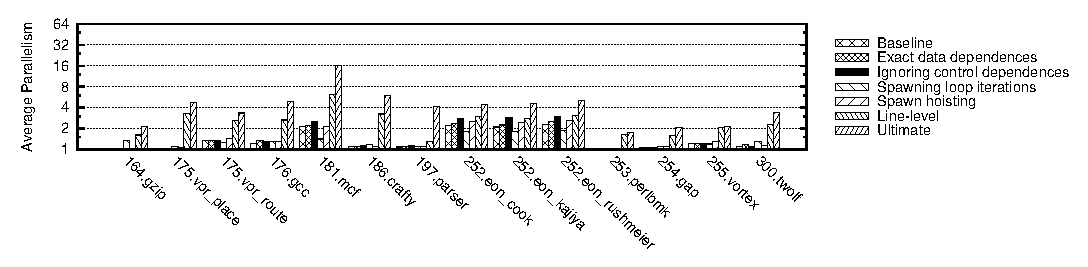
\includegraphics[width=6.5in]{spec}
 \caption{SPEC CPU 2000 integer benchmarks}
 \label{spec}
 \end{subfloat}

 \begin{subfloat}
 \centering
 \includegraphics[width=6.5in]{specfp}
 \caption{SPEC CPU 2000 floating point benchmarks}
 \label{specfp}
 \end{subfloat}

 \begin{subfloat}
 \centering
 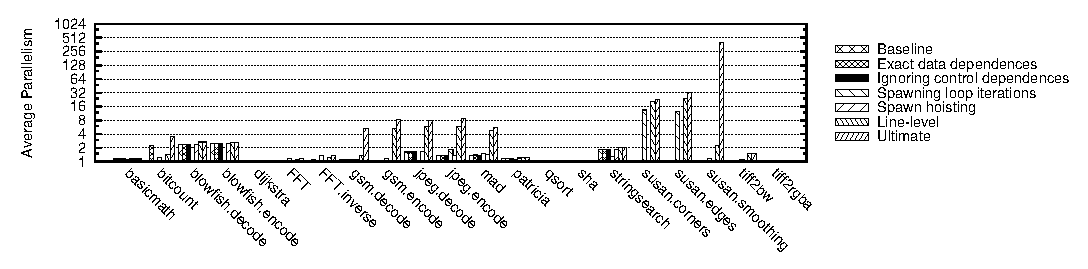
\includegraphics[width=6.5in]{mb}
 \caption{miBench}
 \label{mb}
 \end{subfloat}
\caption{Parallelism of three benchmark suites under various models}
\label{benchmarks}
\end{figure*}

We also ran the same analysis using our tool on some of benchmark programs in the SPEC CPU 2000 (with the MinneSPEC reduced data input set \cite{KleinOsowski02minnespec}) and miBench suites, the results of which are displayed in Figure~\ref{benchmarks}.
As before, the baseline model uses agreegated data dependences and control dependences, and considers only function-call-level parallelism without loop parallelization or spawn hoisting.
Each of the other models differs from the baseline by one parameter described in Section~\ref{smethod}, except for Ultimate, which considers line-level parallelism by using exact data dependences, ignoring control dependences and hoisting spawns.
In general, we see that few benchmarks exhibit the level of parallelism seen in the Cilk examples.
In fact, none of these benchmarks exhibit parallelism of over 3 under the baseline model.

There are, however, some benchmarks with a significant amount of loop-level parallelism.
One of them is the miBench benchmark SUSAN, a program that performs image smoothing, corner detection and edge detection on an image, and is data-parallel---the same computation is performed on each pixel in the image and the results for each pixel are independent of each other.
This is reflected in our results, which show that both susan.corners and susan.edges have potential parallelism of over 12 when loop iterations are spawned.
The same would have been true for susan.smoothing had it not had an associative reduction variable in the loop, which as mentioned our tool currently cannot recognise.

We note also that for some programs, e.g.\ eon, spawning loop iterations actually results in a \emph{lower} level of parallelism.
This is because that while spawning loop iterations allows us to exploit DOALL parallelism, where loop iterations are completely independent from each other and can be executed in parallel, it precludes DOACROSS parallelism or software pipelining, where there are cross-iteration dependences but loop iterations can still partially overlap.
The balance between DOALL and DOACROSS loops would therefore determine whether parallelism rises or falls compared to the baseline.

\subsection{Discussion}

Our results suggest that while the example programs from Cilk have lots of inherent task-level parallelism, most general-purpose programs tend to have little and cannot be transformed into highly concurrent programs simply by spawning existing function calls and loops.
Nevertheless, our extension of Embla can output the critical path of each function call, allowing us to examine the bottlenecks that prevent greater parallelism from being realised.
Having examined several programs in more detail, we now present some of the reasons why they exhibit such low levels of parallelism, and suggest what can be done to increase their potential.

\subsubsection{186.crafty}

Crafty is a chess-playing program that uses a Minimax-like algorithm to find the best move through searching a game tree.
In theory game tree searching is an easily parallelisable activity, as demonstrated by the success of multi-threaded chess-playing programs \cite{Dailey01usingcilk}.
However, our tool does not find plenty of parallelism in Crafty for a number of reasons.
Firstly, Crafty uses one global chessboard, which is updated when a move is considered and then reverted afterwards, creating a chain of data dependences that linearise the search.
Furthermore, various pruning techniques used mean that later searches are influenced by the results of earlier ones.
This shows that algorithmic changes are required before such a program can be parallelized.

\subsubsection{164.gzip}

Gzip is a file compression program.
It works by traversing the input file sequentially, looking for recurrences of substrings that have been seen before.
As such it is easy to see that the program cannot process the later parts of the file before the earlier parts have been processed---this results in little task-level parallelism.
One could imagine changing the algorithm such that a file is divided into blocks that are compressed independently, resulting in greater parallelism at the cost of a larger output file.

\subsubsection{Input/output}

We find that input/output forms a large part of several benchmarks.
In dijkstra, for example, a tenth of the program's sequential execution time is taken up by calls to \texttt{scanf}.
In FFT (miBench), printing the results takes up around 80\% of processing time.
If we assume that input/output is unparallelisable, Amdahl's law would mean that the maximum speed-up, even if we were able to parallelize the rest of the program perfectly, would still be low.
This suggests that for some of the benchmarks examined, a parallel implementation of input/output would be very useful.

\subsubsection{Getting more parallelism from loops}

\begin{figure}
  \centering
  \begin{subfloat}
    \begin{minipage}{3in}
      \begin{verbatim}
for (j = n = 0, seed = rand();
     j < iterations;
     j++, seed += 13) {
  int r = pBitCntFunc[i](seed);
  n += r;
}
      \end{verbatim}
    \end{minipage}%
    \label{orig}
    \caption{Original program}
  \end{subfloat}%
\\
  \begin{subfloat}
    \label{dnc-trans}
    \begin{minipage}{3in}
      \begin{verbatim}
int dc_bitcnts(int start, int n_itrs, int i) {
  if (n_itrs <= 0) return 0;
  if (n_itrs == 1) return pBitCntFunc[i](start);
  else {
    int x,y;
    int half_itrs = n_itrs / 2;
    x = dc_bitcnts(start, half_itrs, i);
    y = dc_bitcnts(start+(half_itrs*13),
          n_itrs - half_itrs, i);
    return x+y;
  }
}

n = dc_bitcnts(seed, iterations, i);
      \end{verbatim}
    \end{minipage}%
    \caption{Transformed program}
  \end{subfloat}%
  \caption{Tranformation of a loop in the bitcount program using divide and conquer.}
  \label{dnc}
\end{figure}

Despite the relatively low figures of parallelism, there are some simple ways of modifying a program to unlock greater parallelism, one of which we present here.
Figure~\ref{dnc} shows a transformation applied to a (slightly adapted) loop in the bitcount benchmark.
In the original program, calls to \texttt{pBitCntFunc[i]} are pure and can be run in parallel with each other.
However, there is a dependence between increments of the induction variables, \texttt{j} and \texttt{seed}, and between additions to the accumulator \texttt{n}, producing two long chains of data dependences.
Nevertheless, by recognising that \texttt{n} is a reduction variable we can transform the loop into recursive calls using a divde-and-conquer strategy.
The lengths of the dependence chains on the induction and reduction variables become logarithmic on the number of iterations instead of linear, and consequently the critical path found by our tool is a tenth of that in the original program, despite the overheads of extra function calls.
This shows that simple transformations can sometimes be sufficient to increase the amount of potential parallelism in certain programs.
In fact, we note that Cilk++, the commercialised version of Cilk, indeed uses a divide-and-conquer strategy for its parallel for-loops, a decision which is justified by our example.

 % 5 pages
\section{Related work}

% Explicit task level parallelism
A lot of languages and libraries have been created to allow easy expression of task-level parallelism.
Cilk's \cite{blumofe96cilk} model of fork/join parallelism matches our function-spawning model most closely, although we find that Cilk only allows joining of all active threads rather than one specific thread.
OpenMP \cite{dagum98openmp}, on the other hand, focuses on loop-level parallelism.
Other notable examples include Java's concurrency library \cite{lea00java} and  X10 \cite{charles05x10}.

% Other limits surveys
Several studies have been made on instruction-level parallelism \cite{wall91limits, postiff99limits, austin92dynamic, lam92limits, mak09limits}, but fewer have tried to separate out task-level parallelism from instruction-level parallelism.
Kreaseck et al. \cite{Kreaseck00limitsof} explored limits of speculative task-level parallelism by pre-emptively executing function calls, similar to the way we hoist spawns.
Warg and Stenstr\"{o}m \cite{warg01limits} focused on finding function-call-level parallelism, with an emphasis on comparing object-oriented programs with ordinary imperative ones.

% Race detection

% Automatic parallelisation

% Thread-level speculation
 % 0.5 page
\section{Conclusions}

We have presented Embla 2, a tool designed to aid manual parallelization by estimating and locating inherent parallelism in programs as well as pinpointing bottlenecks.
It works by profiling dependences and mapping them back to program source.
The underlying model of parallelism treats each function call as a spawnable task, which is synchronized on as late as dependences allow.
Variants of this model allow us to estimate the potential benefits of various optimizations, such as thread-level speculation.

Embla 2 can locate inherent parallelism in programs with lots of it,
as shown by its reconstruction of parallel tasks in the Cilk test suite.
For those without much readily available parallelism,
such as many SPEC CPU 2000 and MiBench benchmarks,
Embla 2 outputs critical paths to assist the programmer in pinpointing bottlenecks and finding solutions.
Some programmer effort is still required to realize task-level parallelism in this case,
and we suggest two extensions to provide further assistance:
one is an IDE that can simplify a critical path down to a regular expression that represents it more succinctly,
and the other is a compiler that can perform code motion to move task-serializing operations,
such as the induction variable update in \textsf{susan.smoothing}, outside task boundaries,
thereby making the tasks independent and hence parallelizable.
All in all, we believe Embla 2 would be a useful aid for programmers parallelizing legacy sequential applications using parallel programming frameworks such as Cilk.
 % 0.5 page

\section*{Acknowledgements}

The first author thanks St John's College, Cambridge for funding his studentship.

\bibliographystyle{abbrv}
\bibliography{bib.bib}{}

\end{document}

